\documentclass[12pt,a4paper]{article}

\usepackage[a4paper,text={16.5cm,25.2cm},centering]{geometry}
\usepackage{lmodern}
\usepackage{amssymb,amsmath}
\usepackage{bm}
\usepackage{graphicx}
\usepackage{microtype}
\usepackage{hyperref}
\setlength{\parindent}{0pt}
\setlength{\parskip}{1.2ex}

\hypersetup
       {   pdfauthor = {  },
           pdftitle={  },
           colorlinks=TRUE,
           linkcolor=black,
           citecolor=blue,
           urlcolor=blue
       }




\usepackage{upquote}
\usepackage{listings}
\usepackage{xcolor}
\lstset{
    basicstyle=\ttfamily\footnotesize,
    upquote=true,
    breaklines=true,
    breakindent=0pt,
    keepspaces=true,
    showspaces=false,
    columns=fullflexible,
    showtabs=false,
    showstringspaces=false,
    escapeinside={(*@}{@*)},
    extendedchars=true,
}
\newcommand{\HLJLt}[1]{#1}
\newcommand{\HLJLw}[1]{#1}
\newcommand{\HLJLe}[1]{#1}
\newcommand{\HLJLeB}[1]{#1}
\newcommand{\HLJLo}[1]{#1}
\newcommand{\HLJLk}[1]{\textcolor[RGB]{148,91,176}{\textbf{#1}}}
\newcommand{\HLJLkc}[1]{\textcolor[RGB]{59,151,46}{\textit{#1}}}
\newcommand{\HLJLkd}[1]{\textcolor[RGB]{214,102,97}{\textit{#1}}}
\newcommand{\HLJLkn}[1]{\textcolor[RGB]{148,91,176}{\textbf{#1}}}
\newcommand{\HLJLkp}[1]{\textcolor[RGB]{148,91,176}{\textbf{#1}}}
\newcommand{\HLJLkr}[1]{\textcolor[RGB]{148,91,176}{\textbf{#1}}}
\newcommand{\HLJLkt}[1]{\textcolor[RGB]{148,91,176}{\textbf{#1}}}
\newcommand{\HLJLn}[1]{#1}
\newcommand{\HLJLna}[1]{#1}
\newcommand{\HLJLnb}[1]{#1}
\newcommand{\HLJLnbp}[1]{#1}
\newcommand{\HLJLnc}[1]{#1}
\newcommand{\HLJLncB}[1]{#1}
\newcommand{\HLJLnd}[1]{\textcolor[RGB]{214,102,97}{#1}}
\newcommand{\HLJLne}[1]{#1}
\newcommand{\HLJLneB}[1]{#1}
\newcommand{\HLJLnf}[1]{\textcolor[RGB]{66,102,213}{#1}}
\newcommand{\HLJLnfm}[1]{\textcolor[RGB]{66,102,213}{#1}}
\newcommand{\HLJLnp}[1]{#1}
\newcommand{\HLJLnl}[1]{#1}
\newcommand{\HLJLnn}[1]{#1}
\newcommand{\HLJLno}[1]{#1}
\newcommand{\HLJLnt}[1]{#1}
\newcommand{\HLJLnv}[1]{#1}
\newcommand{\HLJLnvc}[1]{#1}
\newcommand{\HLJLnvg}[1]{#1}
\newcommand{\HLJLnvi}[1]{#1}
\newcommand{\HLJLnvm}[1]{#1}
\newcommand{\HLJLl}[1]{#1}
\newcommand{\HLJLld}[1]{\textcolor[RGB]{148,91,176}{\textit{#1}}}
\newcommand{\HLJLs}[1]{\textcolor[RGB]{201,61,57}{#1}}
\newcommand{\HLJLsa}[1]{\textcolor[RGB]{201,61,57}{#1}}
\newcommand{\HLJLsb}[1]{\textcolor[RGB]{201,61,57}{#1}}
\newcommand{\HLJLsc}[1]{\textcolor[RGB]{201,61,57}{#1}}
\newcommand{\HLJLsd}[1]{\textcolor[RGB]{201,61,57}{#1}}
\newcommand{\HLJLsdB}[1]{\textcolor[RGB]{201,61,57}{#1}}
\newcommand{\HLJLsdC}[1]{\textcolor[RGB]{201,61,57}{#1}}
\newcommand{\HLJLse}[1]{\textcolor[RGB]{59,151,46}{#1}}
\newcommand{\HLJLsh}[1]{\textcolor[RGB]{201,61,57}{#1}}
\newcommand{\HLJLsi}[1]{#1}
\newcommand{\HLJLso}[1]{\textcolor[RGB]{201,61,57}{#1}}
\newcommand{\HLJLsr}[1]{\textcolor[RGB]{201,61,57}{#1}}
\newcommand{\HLJLss}[1]{\textcolor[RGB]{201,61,57}{#1}}
\newcommand{\HLJLssB}[1]{\textcolor[RGB]{201,61,57}{#1}}
\newcommand{\HLJLnB}[1]{\textcolor[RGB]{59,151,46}{#1}}
\newcommand{\HLJLnbB}[1]{\textcolor[RGB]{59,151,46}{#1}}
\newcommand{\HLJLnfB}[1]{\textcolor[RGB]{59,151,46}{#1}}
\newcommand{\HLJLnh}[1]{\textcolor[RGB]{59,151,46}{#1}}
\newcommand{\HLJLni}[1]{\textcolor[RGB]{59,151,46}{#1}}
\newcommand{\HLJLnil}[1]{\textcolor[RGB]{59,151,46}{#1}}
\newcommand{\HLJLnoB}[1]{\textcolor[RGB]{59,151,46}{#1}}
\newcommand{\HLJLoB}[1]{\textcolor[RGB]{102,102,102}{\textbf{#1}}}
\newcommand{\HLJLow}[1]{\textcolor[RGB]{102,102,102}{\textbf{#1}}}
\newcommand{\HLJLp}[1]{#1}
\newcommand{\HLJLc}[1]{\textcolor[RGB]{153,153,119}{\textit{#1}}}
\newcommand{\HLJLch}[1]{\textcolor[RGB]{153,153,119}{\textit{#1}}}
\newcommand{\HLJLcm}[1]{\textcolor[RGB]{153,153,119}{\textit{#1}}}
\newcommand{\HLJLcp}[1]{\textcolor[RGB]{153,153,119}{\textit{#1}}}
\newcommand{\HLJLcpB}[1]{\textcolor[RGB]{153,153,119}{\textit{#1}}}
\newcommand{\HLJLcs}[1]{\textcolor[RGB]{153,153,119}{\textit{#1}}}
\newcommand{\HLJLcsB}[1]{\textcolor[RGB]{153,153,119}{\textit{#1}}}
\newcommand{\HLJLg}[1]{#1}
\newcommand{\HLJLgd}[1]{#1}
\newcommand{\HLJLge}[1]{#1}
\newcommand{\HLJLgeB}[1]{#1}
\newcommand{\HLJLgh}[1]{#1}
\newcommand{\HLJLgi}[1]{#1}
\newcommand{\HLJLgo}[1]{#1}
\newcommand{\HLJLgp}[1]{#1}
\newcommand{\HLJLgs}[1]{#1}
\newcommand{\HLJLgsB}[1]{#1}
\newcommand{\HLJLgt}[1]{#1}


\begin{document}



\section{Problem 1}
\section{Problem 2}
$\int_1^3 \sqrt(2+\cos(x)^3)\exp(\sin(x))dx$


\begin{lstlisting}
(*@\HLJLk{using}@*) (*@\HLJLn{LinearAlgebra}@*)
(*@\HLJLk{using}@*) (*@\HLJLn{Plots}@*)
(*@\HLJLk{using}@*) (*@\HLJLn{LaTeXStrings}@*)

(*@\HLJLnf{f}@*)(*@\HLJLp{(}@*)(*@\HLJLn{t}@*)(*@\HLJLp{)}@*) (*@\HLJLoB{=}@*) (*@\HLJLnf{sqrt}@*)(*@\HLJLp{(}@*)(*@\HLJLni{2}@*) (*@\HLJLoB{+}@*) (*@\HLJLnf{cos}@*)(*@\HLJLp{(}@*)(*@\HLJLn{t}@*)(*@\HLJLp{)}@*)(*@\HLJLoB{{\textasciicircum}}@*)(*@\HLJLni{3}@*)(*@\HLJLp{)}@*)(*@\HLJLoB{*}@*)(*@\HLJLnf{exp}@*)(*@\HLJLp{(}@*)(*@\HLJLnf{sin}@*)(*@\HLJLp{(}@*)(*@\HLJLn{t}@*)(*@\HLJLp{))}@*)

(*@\HLJLk{function}@*) (*@\HLJLnf{CompTrapezoid}@*)(*@\HLJLp{(}@*)(*@\HLJLn{N}@*)(*@\HLJLp{,}@*) (*@\HLJLn{a}@*)(*@\HLJLp{,}@*) (*@\HLJLn{b}@*)(*@\HLJLp{,}@*) (*@\HLJLn{f}@*)(*@\HLJLp{)}@*)

    (*@\HLJLcm{{\#}=}@*)
        (*@\HLJLcm{Integrates}@*) (*@\HLJLcm{f(t)}@*) (*@\HLJLcm{from}@*) (*@\HLJLcm{a}@*) (*@\HLJLcm{to}@*) (*@\HLJLcm{b}@*) (*@\HLJLcm{using}@*) (*@\HLJLcm{composite}@*) (*@\HLJLcm{trapezoid}@*) (*@\HLJLcm{rule}@*)

        (*@\HLJLcm{Input}@*) (*@\HLJLcm{variables}@*)
        (*@\HLJLcm{N:}@*) (*@\HLJLcm{number}@*) (*@\HLJLcm{of}@*) (*@\HLJLcm{points}@*)
        (*@\HLJLcm{a:}@*) (*@\HLJLcm{initial}@*) (*@\HLJLcm{point}@*)
        (*@\HLJLcm{b:}@*) (*@\HLJLcm{final}@*) (*@\HLJLcm{point}@*)
        (*@\HLJLcm{f:}@*) (*@\HLJLcm{function}@*) (*@\HLJLcm{to}@*) (*@\HLJLcm{be}@*) (*@\HLJLcm{integrated}@*)

        (*@\HLJLcm{local}@*) (*@\HLJLcm{variables}@*)
        (*@\HLJLcm{h:}@*) (*@\HLJLcm{step}@*) (*@\HLJLcm{size}@*)
        (*@\HLJLcm{s:}@*) (*@\HLJLcm{solution}@*)
    (*@\HLJLcm{={\#}}@*)

    (*@\HLJLn{h}@*) (*@\HLJLoB{=}@*) (*@\HLJLp{(}@*)(*@\HLJLn{b}@*)(*@\HLJLoB{-}@*)(*@\HLJLn{a}@*)(*@\HLJLp{)}@*)(*@\HLJLoB{/}@*)(*@\HLJLn{N}@*)
    (*@\HLJLn{s}@*) (*@\HLJLoB{=}@*) (*@\HLJLni{0}@*)
    (*@\HLJLk{for}@*) (*@\HLJLn{i}@*) (*@\HLJLoB{=}@*) (*@\HLJLni{1}@*)(*@\HLJLoB{:}@*)(*@\HLJLn{N}@*)
        (*@\HLJLn{s}@*) (*@\HLJLoB{+=}@*) (*@\HLJLn{h}@*)(*@\HLJLoB{/}@*)(*@\HLJLni{2}@*) (*@\HLJLoB{*}@*) (*@\HLJLp{(}@*)(*@\HLJLnf{f}@*)(*@\HLJLp{(}@*)(*@\HLJLn{a}@*) (*@\HLJLoB{+}@*) (*@\HLJLn{h}@*)(*@\HLJLoB{*}@*)(*@\HLJLp{(}@*)(*@\HLJLn{i}@*)(*@\HLJLoB{-}@*)(*@\HLJLni{1}@*)(*@\HLJLp{))}@*) (*@\HLJLoB{+}@*) (*@\HLJLnf{f}@*)(*@\HLJLp{(}@*)(*@\HLJLn{a}@*) (*@\HLJLoB{+}@*) (*@\HLJLn{h}@*)(*@\HLJLoB{*}@*)(*@\HLJLn{i}@*)(*@\HLJLp{))}@*)
    (*@\HLJLk{end}@*)
    (*@\HLJLk{return}@*) (*@\HLJLn{s}@*)
(*@\HLJLk{end}@*)

(*@\HLJLk{function}@*) (*@\HLJLnf{CompSimpson}@*)(*@\HLJLp{(}@*)(*@\HLJLn{N}@*)(*@\HLJLp{,}@*) (*@\HLJLn{a}@*)(*@\HLJLp{,}@*) (*@\HLJLn{b}@*)(*@\HLJLp{,}@*) (*@\HLJLn{f}@*)(*@\HLJLp{)}@*)

    (*@\HLJLcm{{\#}=}@*)
        (*@\HLJLcm{Integrates}@*) (*@\HLJLcm{f(t)}@*) (*@\HLJLcm{from}@*) (*@\HLJLcm{a}@*) (*@\HLJLcm{to}@*) (*@\HLJLcm{b}@*) (*@\HLJLcm{using}@*) (*@\HLJLcm{composite}@*) (*@\HLJLcm{simpsons}@*) (*@\HLJLcm{rule}@*)

        (*@\HLJLcm{Input}@*) (*@\HLJLcm{variables}@*)
        (*@\HLJLcm{N:}@*) (*@\HLJLcm{number}@*) (*@\HLJLcm{of}@*) (*@\HLJLcm{points}@*)
        (*@\HLJLcm{a:}@*) (*@\HLJLcm{initial}@*) (*@\HLJLcm{point}@*)
        (*@\HLJLcm{b:}@*) (*@\HLJLcm{final}@*) (*@\HLJLcm{point}@*)
        (*@\HLJLcm{f:}@*) (*@\HLJLcm{function}@*) (*@\HLJLcm{to}@*) (*@\HLJLcm{be}@*) (*@\HLJLcm{integrated}@*)

        (*@\HLJLcm{local}@*) (*@\HLJLcm{variables}@*)
        (*@\HLJLcm{h:}@*) (*@\HLJLcm{step}@*) (*@\HLJLcm{size}@*)
        (*@\HLJLcm{s:}@*) (*@\HLJLcm{solution}@*)
        (*@\HLJLcm{ts:}@*) (*@\HLJLcm{partition}@*) (*@\HLJLcm{points}@*)
    (*@\HLJLcm{={\#}}@*)

    (*@\HLJLn{h}@*) (*@\HLJLoB{=}@*) (*@\HLJLp{(}@*)(*@\HLJLn{b}@*)(*@\HLJLoB{-}@*)(*@\HLJLn{a}@*)(*@\HLJLp{)}@*)(*@\HLJLoB{/}@*)(*@\HLJLn{N}@*)
    (*@\HLJLn{s}@*) (*@\HLJLoB{=}@*) (*@\HLJLnf{f}@*)(*@\HLJLp{(}@*)(*@\HLJLn{a}@*)(*@\HLJLp{)}@*) (*@\HLJLoB{+}@*) (*@\HLJLnf{f}@*)(*@\HLJLp{(}@*)(*@\HLJLn{b}@*)(*@\HLJLp{)}@*)

    (*@\HLJLn{ts}@*) (*@\HLJLoB{=}@*) (*@\HLJLn{a}@*)(*@\HLJLoB{:}@*)(*@\HLJLn{h}@*)(*@\HLJLoB{:}@*)(*@\HLJLn{b}@*)
    (*@\HLJLk{for}@*) (*@\HLJLn{i}@*) (*@\HLJLoB{=}@*) (*@\HLJLni{1}@*)(*@\HLJLoB{:}@*)(*@\HLJLp{(}@*)(*@\HLJLnf{Int}@*)(*@\HLJLp{(}@*)(*@\HLJLn{N}@*)(*@\HLJLoB{/}@*)(*@\HLJLni{2}@*)(*@\HLJLp{)}@*) (*@\HLJLoB{-}@*) (*@\HLJLni{1}@*)(*@\HLJLp{)}@*)
       (*@\HLJLn{s}@*) (*@\HLJLoB{+=}@*) (*@\HLJLni{2}@*)(*@\HLJLoB{*}@*)(*@\HLJLnf{f}@*)(*@\HLJLp{(}@*)(*@\HLJLn{ts}@*)(*@\HLJLp{[}@*)(*@\HLJLni{2}@*)(*@\HLJLoB{*}@*)(*@\HLJLn{i}@*)(*@\HLJLp{])}@*)
    (*@\HLJLk{end}@*)
    (*@\HLJLk{for}@*) (*@\HLJLn{i}@*) (*@\HLJLoB{=}@*) (*@\HLJLni{1}@*)(*@\HLJLoB{:}@*)(*@\HLJLnf{Int}@*)(*@\HLJLp{(}@*)(*@\HLJLn{N}@*)(*@\HLJLoB{/}@*)(*@\HLJLni{2}@*)(*@\HLJLp{)}@*)
        (*@\HLJLn{s}@*) (*@\HLJLoB{+=}@*) (*@\HLJLni{4}@*)(*@\HLJLoB{*}@*)(*@\HLJLnf{f}@*)(*@\HLJLp{(}@*)(*@\HLJLn{ts}@*)(*@\HLJLp{[}@*)(*@\HLJLni{2}@*)(*@\HLJLoB{*}@*)(*@\HLJLn{i}@*)(*@\HLJLoB{-}@*)(*@\HLJLni{1}@*)(*@\HLJLp{])}@*)
    (*@\HLJLk{end}@*)

    (*@\HLJLn{s}@*) (*@\HLJLoB{=}@*) (*@\HLJLn{h}@*)(*@\HLJLoB{/}@*)(*@\HLJLni{3}@*) (*@\HLJLoB{*}@*) (*@\HLJLn{s}@*)
    (*@\HLJLk{return}@*) (*@\HLJLn{s}@*)
(*@\HLJLk{end}@*)

(*@\HLJLn{a}@*) (*@\HLJLoB{=}@*) (*@\HLJLni{1}@*)(*@\HLJLp{;}@*) (*@\HLJLn{b}@*) (*@\HLJLoB{=}@*) (*@\HLJLni{3}@*)(*@\HLJLp{;}@*) (*@\HLJLn{T}@*) (*@\HLJLoB{=}@*) (*@\HLJLn{b}@*)(*@\HLJLoB{-}@*)(*@\HLJLn{a}@*)(*@\HLJLp{;}@*)

(*@\HLJLcs{{\#}}@*) (*@\HLJLcs{CompTrapezoid(N,a,b,f)}@*)
(*@\HLJLcs{{\#}}@*) (*@\HLJLcs{CompSimpson(N,a,b,f)}@*)

(*@\HLJLcs{{\#}}@*) (*@\HLJLcs{Plotting}@*) (*@\HLJLcs{error}@*) (*@\HLJLcs{routine}@*)
(*@\HLJLn{NList}@*) (*@\HLJLoB{=}@*) (*@\HLJLni{2}@*) (*@\HLJLoB{.{\textasciicircum}}@*)(*@\HLJLp{(}@*)(*@\HLJLni{2}@*)(*@\HLJLoB{:}@*)(*@\HLJLni{10}@*)(*@\HLJLp{)}@*)
(*@\HLJLn{errTrapeList}@*) (*@\HLJLoB{=}@*) (*@\HLJLnf{zeros}@*)(*@\HLJLp{(}@*)(*@\HLJLnf{size}@*)(*@\HLJLp{(}@*)(*@\HLJLn{NList}@*)(*@\HLJLp{))}@*)
(*@\HLJLn{errSimpList}@*) (*@\HLJLoB{=}@*) (*@\HLJLnf{zeros}@*)(*@\HLJLp{(}@*)(*@\HLJLnf{size}@*)(*@\HLJLp{(}@*)(*@\HLJLn{NList}@*)(*@\HLJLp{))}@*)
(*@\HLJLk{for}@*) (*@\HLJLn{i}@*) (*@\HLJLoB{=}@*) (*@\HLJLni{1}@*) (*@\HLJLoB{:}@*) (*@\HLJLnf{length}@*)(*@\HLJLp{(}@*)(*@\HLJLn{NList}@*)(*@\HLJLp{)}@*)
    (*@\HLJLn{N}@*) (*@\HLJLoB{=}@*) (*@\HLJLn{NList}@*)(*@\HLJLp{[}@*)(*@\HLJLn{i}@*)(*@\HLJLp{]}@*)

    (*@\HLJLn{utrape}@*) (*@\HLJLoB{=}@*) (*@\HLJLnf{CompTrapezoid}@*)(*@\HLJLp{(}@*)(*@\HLJLn{N}@*)(*@\HLJLp{,}@*)(*@\HLJLn{a}@*)(*@\HLJLp{,}@*)(*@\HLJLn{b}@*)(*@\HLJLp{,}@*)(*@\HLJLn{f}@*)(*@\HLJLp{)}@*)
    (*@\HLJLn{utexact}@*) (*@\HLJLoB{=}@*) (*@\HLJLnf{CompTrapezoid}@*)(*@\HLJLp{(}@*)(*@\HLJLni{2}@*)(*@\HLJLoB{*}@*)(*@\HLJLn{N}@*)(*@\HLJLp{,}@*)(*@\HLJLn{a}@*)(*@\HLJLp{,}@*)(*@\HLJLn{b}@*)(*@\HLJLp{,}@*)(*@\HLJLn{f}@*)(*@\HLJLp{)}@*)

    (*@\HLJLn{usimps}@*) (*@\HLJLoB{=}@*) (*@\HLJLnf{CompSimpson}@*)(*@\HLJLp{(}@*)(*@\HLJLn{N}@*)(*@\HLJLp{,}@*)(*@\HLJLn{a}@*)(*@\HLJLp{,}@*)(*@\HLJLn{b}@*)(*@\HLJLp{,}@*)(*@\HLJLn{f}@*)(*@\HLJLp{)}@*)
    (*@\HLJLn{usexact}@*) (*@\HLJLoB{=}@*) (*@\HLJLnf{CompSimpson}@*)(*@\HLJLp{(}@*)(*@\HLJLni{2}@*)(*@\HLJLoB{*}@*)(*@\HLJLn{N}@*)(*@\HLJLp{,}@*)(*@\HLJLn{a}@*)(*@\HLJLp{,}@*)(*@\HLJLn{b}@*)(*@\HLJLp{,}@*)(*@\HLJLn{f}@*)(*@\HLJLp{)}@*)

    (*@\HLJLcs{{\#}}@*) (*@\HLJLcs{errTrapeList[i]}@*) (*@\HLJLcs{=}@*) (*@\HLJLcs{norm(utrape-uexact)}@*)
    (*@\HLJLn{errTrapeList}@*)(*@\HLJLp{[}@*)(*@\HLJLn{i}@*)(*@\HLJLp{]}@*) (*@\HLJLoB{=}@*) (*@\HLJLnf{abs}@*)(*@\HLJLp{(}@*)(*@\HLJLn{utrape}@*)(*@\HLJLoB{-}@*)(*@\HLJLn{utexact}@*)(*@\HLJLp{)}@*)(*@\HLJLoB{./}@*)(*@\HLJLp{(}@*)(*@\HLJLni{1}@*)(*@\HLJLoB{-}@*)(*@\HLJLp{(}@*)(*@\HLJLni{1}@*)(*@\HLJLoB{/}@*)(*@\HLJLni{2}@*)(*@\HLJLoB{{\textasciicircum}}@*)(*@\HLJLni{2}@*)(*@\HLJLp{))}@*)
    (*@\HLJLn{errSimpList}@*)(*@\HLJLp{[}@*)(*@\HLJLn{i}@*)(*@\HLJLp{]}@*) (*@\HLJLoB{=}@*) (*@\HLJLnf{abs}@*)(*@\HLJLp{(}@*)(*@\HLJLn{usimps}@*)(*@\HLJLoB{-}@*)(*@\HLJLn{usexact}@*)(*@\HLJLp{)}@*)(*@\HLJLoB{./}@*)(*@\HLJLp{(}@*)(*@\HLJLni{1}@*)(*@\HLJLoB{-}@*)(*@\HLJLp{(}@*)(*@\HLJLni{1}@*)(*@\HLJLoB{/}@*)(*@\HLJLni{2}@*)(*@\HLJLoB{{\textasciicircum}}@*)(*@\HLJLni{4}@*)(*@\HLJLp{))}@*)
(*@\HLJLk{end}@*)

(*@\HLJLnf{plot}@*)(*@\HLJLp{(}@*)(*@\HLJLn{T}@*)(*@\HLJLoB{./}@*)(*@\HLJLn{NList}@*)(*@\HLJLp{,}@*) (*@\HLJLn{errTrapeList}@*)(*@\HLJLp{,}@*)(*@\HLJLn{label}@*)(*@\HLJLoB{=}@*)(*@\HLJLs{"{}Trapezoid"{}}@*)(*@\HLJLp{,}@*)(*@\HLJLn{xaxis}@*)(*@\HLJLoB{=:}@*)(*@\HLJLn{log}@*)(*@\HLJLp{,}@*)(*@\HLJLn{yaxis}@*)(*@\HLJLoB{=:}@*)(*@\HLJLn{log}@*)(*@\HLJLp{,}@*) (*@\HLJLn{marker}@*) (*@\HLJLoB{=}@*) (*@\HLJLp{(}@*)(*@\HLJLsc{:dot}@*)(*@\HLJLp{,}@*)(*@\HLJLni{5}@*)(*@\HLJLp{),}@*) (*@\HLJLn{add{\_}marker}@*) (*@\HLJLoB{=}@*) (*@\HLJLkc{true}@*)(*@\HLJLp{)}@*)
(*@\HLJLnf{plot!}@*)(*@\HLJLp{(}@*)(*@\HLJLn{T}@*)(*@\HLJLoB{./}@*)(*@\HLJLn{NList}@*)(*@\HLJLp{,}@*) (*@\HLJLn{errSimpList}@*)(*@\HLJLp{,}@*)(*@\HLJLn{label}@*)(*@\HLJLoB{=}@*)(*@\HLJLs{"{}Simpson"{}}@*)(*@\HLJLp{,}@*)(*@\HLJLn{xaxis}@*)(*@\HLJLoB{=:}@*)(*@\HLJLn{log}@*)(*@\HLJLp{,}@*)(*@\HLJLn{yaxis}@*)(*@\HLJLoB{=:}@*)(*@\HLJLn{log}@*)(*@\HLJLp{,}@*) (*@\HLJLn{marker}@*) (*@\HLJLoB{=}@*) (*@\HLJLp{(}@*)(*@\HLJLsc{:square}@*)(*@\HLJLp{,}@*)(*@\HLJLni{5}@*)(*@\HLJLp{),}@*) (*@\HLJLn{add{\_}marker}@*) (*@\HLJLoB{=}@*) (*@\HLJLkc{true}@*)(*@\HLJLp{)}@*)
(*@\HLJLnf{xlabel!}@*)(*@\HLJLp{(}@*)(*@\HLJLso{L"{}h"{}}@*)(*@\HLJLp{)}@*)
(*@\HLJLnf{ylabel!}@*)(*@\HLJLp{(}@*)(*@\HLJLs{"{}Approximate}@*) (*@\HLJLs{Error"{}}@*)(*@\HLJLp{)}@*)
\end{lstlisting}

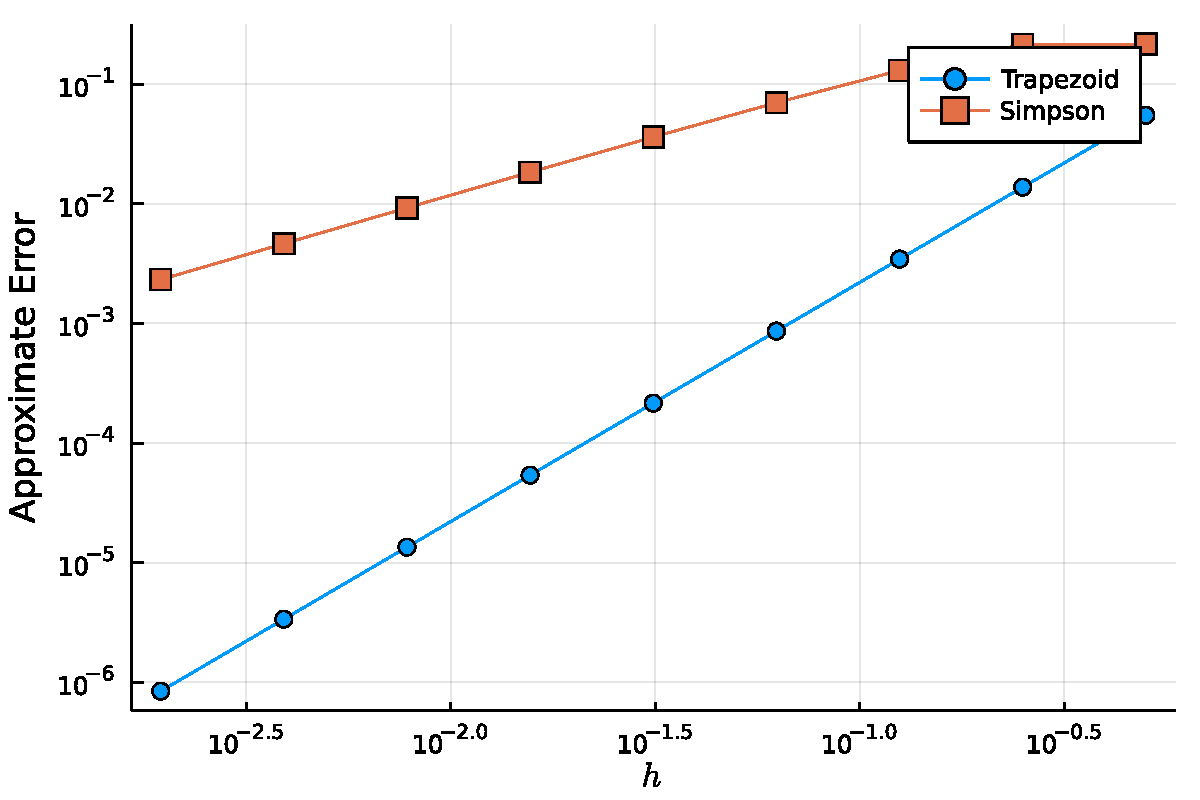
\includegraphics[width=\linewidth]{figures/ass_1_report_1_1.pdf}


\end{document}
